\chapter[Swarm Intelligence]{Metaheuristic Algorithms: Swarm Intelligence}
\label{chpt:swarm}
\section{Introduction}
The research field of artificial intelligence stands a lot to gain by the study of the inner workings of nature itself; this is why there is a branch of artificial intelligence that incorporates some of nature's processes, like evolution, which can be seen being applied in practice in the GA (see section \ref{sec:geneticalgorithm}).

 There are other approaches in artificial intelligence which also have their routes in nature, for instance animal learning or the study of how dogs learn\cite{DLearning}. These approaches only look at a “single agent” thought process when an agent percepts (senses) are mapped to actions in the agents particular environment \cite{DLearning}. 
 
 A percept can be said to be a process that is specifically designed to take data from the surrounding environment, process it and present it as information upon which decisions can be made\cite{DLearning,AIModernApproach}. For instance, eyes are percepts, which take visual data presented by the environment\cite{DLearning,AIModernApproach}. The visual data is processed by the brain into information to enable decisions to be made on navigating the environment\cite{DLearning,AIModernApproach}.

The research field of swarm intelligence is an approach more concerned with the underlying processes and behaviour patterns when multiple agents (insects, animals) come together and perform a task as one collective entity\cite{DLearning,AIModernApproach,ChaoticSwarmIntel,BeeJobShop}.  The study of animals and insects and how they socially interact within their local environments in groups has already contributed to artificial intelligence as a whole in the form of Swarm Intelligence\cite{ChaoticSwarmIntel,BeeJobShop}.  In the field of Swarm Intelligence, animals and insects are represented by agents which are simple stimulus-response agents and can only perceive changes in their local environments. A group of agents is referred to as a \emph{swarm}.

Swarm intelligence works on a key aspect observed in nature, the notion of emergent behaviour\cite{SwarmArt,CompuIntelligenceIntro,FundamentalSwarm}. Emergent behaviour is when an individual in the swarm achieves success due to the it obtaining more knowledge through exploration about its local environment\cite{SwarmArt,CompuIntelligenceIntro,FundamentalSwarm}.

In swarm intelligence, when an agent exhibits emergent behaviour, the outcome of the behaviour needs to be shared with the whole swarm in order for the swarm to adapt and use the newly gained knowledge\cite{SwarmArt,ChaoticSwarmIntel,CompuIntelligenceIntro,FundamentalSwarm}.

In a swarm, the agents communicate with each other about knowledge gained as a consequence of the changes in their local environments\cite{SwarmArt,ChaoticSwarmIntel,CompuIntelligenceIntro,FundamentalSwarm}. Changes can be caused by emergent behaviour by the agent itself, other agents or the environment\cite{SwarmArt,ChaoticSwarmIntel,CompuIntelligenceIntro,FundamentalSwarm}. Communication among agents facilitates \emph{knowledge sharing}\cite{SwarmArt,ChaoticSwarmIntel,CompuIntelligenceIntro,FundamentalSwarm}. 

Social interaction among agents is certainly not the only means of interacting, but with regard to biological inspired systems it is the most prominent\cite{CompuIntelligenceIntro}.

Using this social interaction between the agents of the swarm can influence their own local environment to move towards more promosing space in the search space \cite{SwarmArt,ChaoticSwarmIntel,CompuIntelligenceIntro,FundamentalSwarm}. Due to the social interaction between agents the swarm is also referred to as a \emph{social swarm}\cite{SwarmArt,ChaoticSwarmIntel,CompuIntelligenceIntro,FundamentalSwarm}. Thus each agents of a swarm contributes to the swarm as a whole to locate and produce better solutions \cite{BeeJobShop}. 

As discussed the behaviour propagates from one agent to another through social interaction, which brings forth information exchange\cite{SwarmArt}. Social interaction is but one component of self-organisation. Other components that form part of self-organisation are \cite{SIPowerInNums}:
\begin{itemize}
\item Positive and negative feedback\cite{SIPowerInNums}
\item Increasing fluctuations of random events\cite{SIPowerInNums}
\end{itemize}

The means by which agents facilitate indirect communication with each other is known as \emph{stigmergy}. Stimergy as well as the different forms of stigmergy is discussed in ~\ref{sec:stigmergy}.

Swarm intelligence algorithms are also meta-heuristic algorithms, with the distinction being made that swarm intelligence algorithms use multiple agents as a collective entity of knowledge to search the problem space\cite{SwarmArt,ChaoticSwarmIntel,BeeJobShop,CompuIntelligenceIntro,FundamentalSwarm}.

The initial algorithms developed with regard to swarm intelligence, were based on the coordination and behaviour exhibited by schools of fish and flocks of birds. The newer generation of algorithms include\cite{SwarmArt,ChaoticSwarmIntel,BeeJobShop}:
\begin{itemize}
\item ant colony optimisation (ACO)\cite{SwarmArt}.
\item artificial bee colony (ABC) optimisation\cite{BeeJobShop}.
\item particle swarm optimisation (PSO)\cite{ChaoticSwarmIntel}. 
\item bacterial foraging optimisation\cite{CompuIntelligenceIntro}.
\item Firefly optimisation\cite{CompuIntelligenceIntro}.
\item Fish school optimisation\cite{CompuIntelligenceIntro}.
\end{itemize}


Swarm intelligence based algorithms are able to achieve good results since they have simple individuals searching in their own local environments for more optimal solutions\cite{CompuIntelligenceIntro,FundamentalSwarm}. A direct consequence of multiple individuals in a swarm searching is that the algorithms are able to explore multple locations within the defined search space\cite{CompuIntelligenceIntro,FundamentalSwarm}.Traditional single agent based metaheuristic algorithms like TS (section~\ref{sec:tabusearch}) and SA (section~\ref{sec:simulatedannealing}) only have in essence one ``individual'' searching for a solution\cite{CompuIntelligenceIntro,FundamentalSwarm}. 

With algorithms like TS and SA, the information is not shared since there is only one individual search\cite{CompuIntelligenceIntro,FundamentalSwarm,SASingleMultiObj,TSHazardous}. The information is kept to influence future decisions\cite{AIModernApproach,TabuMontemanniSmith,TabuVechicleRoutingWithTimeWindows,CurveFittingSA,EcoEquilSA}. Swarm intelligence algorithms also store information for use by the various individuals that make up the swarm to make more informed decisions as the solution space is explored\cite{CompuIntelligenceIntro,FundamentalSwarm}.

NP-Complete optimisation problems are but one of the fields where swarm intelligence algorithms have been adapted to. Other fields where swarm intelligence has been applied include neural network training\cite{CompuIntelligenceIntro}, vehicle routing\cite{ACOSurvey}, clustering\cite{AntSwarmClustering}, search engines and electrical power systems\cite{SAElectricPower}. Swarm intelligence thus seems more suited towards problems with combinatorial complexity\cite{SIOPDenby}.

The chapter is organised as follows. Before the algorithms are discussed an overview of stigmergy is presented in section~\ref{sec:stigmergy}. Starting with section~\ref{sec:ACO} the first swarm intelligence algorithm is discussed namely, Ant Colony Optimisation. Artificial bee colony is discussed in section~\ref{sec:BEE}. Section~\ref{sec:PSO} is a discussion about the Particle Swarm Optimisation algorithm. This chapter concludes with section~\ref{sec:SISummary} that summurises the chapter.

\section{Stigmergy}
\label{sec:stigmergy}
Stigmergy is defined as the method used by animals and insects to facilitate indirect communication\cite{AntsAndStigmergy,CompuIntelligenceIntro,AntIntroTrends,FundamentalSwarm}. Through the use of stimergy animals or insects are able to socially interact with their own species to convey information to each other\cite{AntsAndStigmergy,CompuIntelligenceIntro,AntIntroTrends,FundamentalSwarm}.

Interaction occurs through signals that the individuals receive which might require them to perform a specific action\cite{AntsAndStigmergy,CompuIntelligenceIntro,AntIntroTrends}.

Two forms of stigmergy can be observed in nature. One form, \emph{sematectonic stigmergy}\label{def:sematectonic}, is a direct and physical form of interaction since it relies on altering the environment\cite{CompuIntelligenceIntro}. 

Examples of this type of stigmergy are nest building and brood sorting by ants\cite{CompuIntelligenceIntro}. Schools of fish also use this type of stigmergy to communicate direction and speed by visually observing their closest partner in the school. Besides using visual information, birds use sound to communicate with and alert each other\cite{SwarmArt}.

The other form, \emph{sign-based stigmergy}, is an indirect form of interaction, where communication occurs through some sort of signal mechanism\cite{CompuIntelligenceIntro}. Ants use sign-based stigmergy to communicate with each other. More on how ants communicate with this type of stigmergy is discussed in section~\ref{sec:ACOverview}.

Other species that use sign-based stigmergy are bees\cite{stigmergicoptimization}. When a bee determines that an entity poses a threat to the hive, it might decide to sting the entity. The sting of a bee not only injects a toxin into the entity, but also releases a pheromone\cite{stigmergicoptimization}. This pheromone alerts nearby other bees from the hive of the presence of an entity that is a potential danger to the hive\cite{stigmergicoptimization}. 

The other bees of the hive pick up this pheromone that is released by the initial bee's stinger and attack the entity by also stinging it\cite{stigmergicoptimization}. As more bees sting the entity, more bee stingers emit the danger pheromone identifying the entity\cite{stigmergicoptimization}. Hence the pheromone is reinforced and becomes stronger, which persuades more bees into action\cite{stigmergicoptimization}.

Stigmergy is a powerful mechanism that is able to alter the behaviour of a collective entity efficiently, as can be gathered from the above-mentioned examples of stigmergy in nature\cite{AntsAndStigmergy,CompuIntelligenceIntro,AntIntroTrends}. Stigmergy is therefore a core concept upon which swarm intelligence algorithms are based as these communication techniques are exploited to aid the algorithm in finding better solutions\cite{AntsAndStigmergy,CompuIntelligenceIntro,AntIntroTrends}.

In the forthcoming sections three swarm intelligence algorithms is discussed. Each section is divided into four subsections. 

First, an overview of the algorithm is given, where basic concepts about the algorithm are introduced as well as a general outline given of the search process the algorithm uses. 
The second subsection will give an in-depth discussion of some of the core characteristics that make the algorithm unique. 
The third subsection will provide a step-by-step discussion of the algorithm using pseudocode as a reference.

Finally, for each algorithm studies using the algorithm on the FAP are mentioned and the various considerations that need to be made to apply the algorithm to the FAP are identified.

\section{Ant Colony Optimisation (ACO)}
\label{sec:ACO}
\subsection{Introduction}
\label{sec:ACOverview}
ACO is a class of algorithms incorporating different behavioural aspects that ants exhibit when they perform certain activities, i.e. gather food, build nests and construct cemeteries\cite{AntsAndStigmergy,CompuIntelligenceIntro}. The first ACO algorithms that were developed were based on the foraging behaviour that was exhibited by ants when finding the most optimal path towards a food source. Deneubourg noticed the foraging behaviour when he performed the bridge experiment \cite{AntsAndStigmergy,CompuIntelligenceIntro}.

The bridge experiment outlined by Deneubourg placed a food source a certain distance away from the nest\cite{AntsAndStigmergy,CompuIntelligenceIntro}. Two bridges of equal length were established towards the food resource. The ants initially selected a path randomly with no clear distinction of the more dominant path to take to retrieve food from the food source\cite{AntsAndStigmergy,CompuIntelligenceIntro}. After a finite amount of time, one of paths to the food source became the preferred route for the ants even though both paths were of equal length. The preference of the one bridge by the ants is due to the bridge having a higher concentration of pheromones due to the bridge being chosen randomly more by ants. 

The bridge experiment was extended to have two bridges that differ in length. The extended bridge experiment is presented in figure~\ref{fig:antBridgeExperiment} and is known as the shortest path bridge experiement\cite{FundamentalSwarm}. In this experiment the ants started to prefer the shortest bridge within a finite amount of time\cite{FundamentalSwarm}. The conclusion was made that the ants prefered the shorter bridge because ants return to the nest quicker and therefore the path is reinforced with pheromones faster than on the longer path\cite{FundamentalSwarm}.

\begin{figure}[H]
	\centering
	\setlength \fboxsep{0pt}
	\setlength \fboxrule{0.5pt}
	\fbox{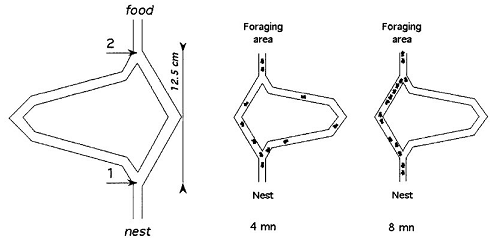
\includegraphics[width=4.0in,height=2.0in]{./pictures/antBridgeExperiment.png}}
	\caption{The shortest path bridge experiment \cite{AntsAndStigmergy}}
	\label{fig:antBridgeExperiment}
\end{figure}
Deneubourg concluded that ants utilise pheromones to communicate to the rest of the foraging ants the shortest path towards a food source.\cite{FundamentalSwarm} By using pheromones to communicate with other ants it can be concluded that ants use sign-based stigmergy (discussed in section~\ref{sec:stigmergy}) when they retrieve food\cite{AntIntroTrends,AntsAndStigmergy,CompuIntelligenceIntro}. As the ant moves along a particular path, it marks the path with a chemical signal that alerts other ants to the desirability of the path \cite{CompuIntelligenceIntro}. The chemical signal that ants use to indicate optimal paths is called \emph{pheromones}\cite{AntsAndStigmergy,CompuIntelligenceIntro}.

Pheromones used by the ACO go through two phases. The first phase is where pheromones a despoited on a particular path by an ant whether their exists previous pheromones or not. The second phase is where pheromones evapurate. Pheromones are not permenant and deteriorate over time\cite{FundamentalSwarm}. By letting pheromones evapurate, ants can ``forget'' previous desicions made by die colony\cite{FundamentalSwarm}. It can be concluded that the more pheromones evapurate the less influence the ants will have on their path selection, therefore promoting exploration\cite{FundamentalSwarm}.

The concept of pheromones and how the ACO proceeds in updating the pheromones is a critical concept of ACO. Hence, an in-depth discussion on pheromones is provided in subsection \ref{sec:ACOcharacter}.

The ACO class of algorithms have a \emph{core requirement} about the problem they are applied to\cite{FundamentalSwarm}. The problem must be able to be modelled as a graph. The reason behind this requirement is that each individial ant in the ACO algorithm constructs a path through the graph\cite{FundamentalSwarm}. The path constructed represents a solution.

A path through a graph is made up of a series of links between nodes\cite{AIModernApproach,DataStructuresJava}. A link between two nodes represents a movement from one node to the other\cite{AIModernApproach,DataStructuresJava}. Therefore, a path can be considered as the traversal of the interlinked nodes, from a starting node to some final node\cite{AIModernApproach,DataStructuresJava}. A path differs from another path by the order in which the nodes are interlinked between a start and end node\cite{AIModernApproach,DataStructuresJava}.

 The ACO class of algorithms has been applied to a wide range of problems that include single machine scheduling\cite{ACOSingleMachine},weapon target assignment\cite{WeaponTargetACO}, flow shop scheduling\cite{ACOFlowShop} and image thresholding\cite{ACOImageThreshold}. Variants of the standard algorithm have been developed, but all of the algorithms still follow the core structure of the ACO algorithm\cite{CompuIntelligenceIntro,FundamentalSwarm}.
The first algorithm developed based on the foraging behaviour of ants is known as the \emph{simple} ACO (SACO) and was proposed by Dorigo in 1992 \cite{CompuIntelligenceIntro}. The algorithm provided the basis for how pheromones are used and updated. The SACO is an algorithmic implementation of the double bridge experiment.

The first algorithm to improve upon the SACO is the ants system (AS) \cite{CompuIntelligenceIntro,AntIntroTrends}. The AS included heuristic information into the probability that an ants chooses to move towards a node. The AS also added memory to the AS by using a tabu list and also incorporated pheromone evapuration. The improvements made enabled the AS to better explore the search space and produce better results\cite{CompuIntelligenceIntro,AntIntroTrends}. 

The AS algorithm has achieved relatively good success in the problems it has been applied to, but it does have some disadvantages\cite{ImpACOComplex,ACOSurvey}. One of the primary disadvantages of AS is that it tends to prematuve converge on local optima \cite{FundamentalSwarm,ImpACOComplex}. The premature convergence can be attributed to due to the ants exploiting the high concentration of pheromones on good solution paths too quickly\cite{FundamentalSwarm}. With the ants focusing only on the good solutions less exploration occurs in the search space leading to local optima being produced as the best solution\cite{FundamentalSwarm}.

Subsequently, various algorithms have been developed that improve on the AS algorithm. These improved algorithms include the ant colony system (ACS), max-min ant system, Ant-Q, fast ant system, AntTabu, AS-rank and approximated non-deterministic tree search (ANTS) \cite{CompuIntelligenceIntro,AntIntroTrends}. The discussion in this section is focused on providing an introduction to the general ACO algorithm concepts and not to discuss various improvements made by variants of the core algorithm. In the forth coming sections reference is made to these algorithms and their respective improvements.

The AS algorithm is the base algorithm upon which all other ACO class algorithms are based upon. Therefore in the forth coming sections when a reference is made to the ACO algorithm it is directed at the base AS algorithm.

In this section the concepts  upon which the core of ACO is based upon were briefly introduced. The concepts include pheromone trails, pheromone evapuration, pheromone updating and state transition rules. In the next section a discussion is given on each of the concepts.
\subsection{ACO Characteristics}
\label{sec:ACOcharacter}
In this section characteristics that are important and unique to the ACO class of algorithms is discussed. The discussion is focused upon three core characteristics namely pheromone trials, pheromone evaporation, pheromone updates and state transition rules.
\subsubsection{Pheromone Trail}
\label{sec:pheromonetrail}
The pheromone technique used by ants forms part of the core methodology used by the ACO algorithm \cite{AntQAP}. As an ant moves it lays down pheromones to mark the path it is walking.

With the use of pheromones ants are able to communicate the best and shortest link between nodes\cite{AntQAP,AntsAndStigmergy,CompuIntelligenceIntro}. The more ants following a preferred link the more pheromones would be laid on that specific link. This increases the strength of the pheromones \cite{ImpACOComplex}. The increase in strength of the pheromones on a link would thus let ants more clearly distinguish between links they should and should not take \cite{ImpACOComplex}. Therefore, a pheromone provides positive feedback to the colony\cite{AntQAP,AntsAndStigmergy,CompuIntelligenceIntro}.

Initially, all the ants will choose random a link to a node\cite{AntQAP,AntsAndStigmergy,CompuIntelligenceIntro}. After all the ants have completed their paths, each path is evaluated using a cost function defined by the problem domain\cite{CompuIntelligenceIntro}. The amount of pheromone marking the links contained in a path in the standard ACO is related to the cost function\cite{AntQAP,AntsAndStigmergy,CompuIntelligenceIntro}. Therefore, a low cost function value will have a high pheromone dosage indicating the link the ant took from each node, and a high cost function value will have a low dosage\cite{CompuIntelligenceIntro}. 


By incorporating the cost of a particular path into the amount of pheromone deposited the colony is able to influcence future decisions\cite{CompuIntelligenceIntro}. In terms of minimisation a path with a low cost will have a high pheromone value making the links of path more likely to be selected by future ants\cite{CompuIntelligenceIntro}.

In the iterations following the initial one, the ants will at each node decide based on a probability whether it should to a particular neighbouring node. The higher the pheromone intensity is at a neighbouring node, the higher the probability that the ant will choose to move towards that node\cite{AntQAP,AntsAndStigmergy,CompuIntelligenceIntro}. The probability with which ants choose links to neighbouring nodes will defined and discussed in the next section.

Due ants choosing links to node based on a probability, it is still possible for the ant to choose a random link towards an other node. Thus the ACO algorithms are considered stochastic search proceduresdue to the ants ability to choose links randomly when exploring the search space \cite{ACOSurvey,ImpACOComplex}.

The pheromone trail was initially developed with only one colony in mind \cite{CompuIntelligenceIntro}. In the research done by Tiwari et al.\cite{ACOLargeProblem} pheromones in multiple colonies are considered. The basic principle of how pheromones are used by the ants stays the same, but the meaning of the pheromone changes if an ant of another colony encounters the pheromone trail\cite{AntQAP,AntsAndStigmergy,CompuIntelligenceIntro}. The ant will not follow or even consider the pheromone trail since any pheromone encountered from other colonies repulses the ant\cite{ACOLargeProblem}. Thus pheromones only provide positive feedback if the ant is from the same colony, otherwise the pheromone gives negative feedback, in a way warning the ant to stay away\cite{ACOLargeProblem}. This repulsion strategy promotes exploration among the multiple colonies\cite{ACOLargeProblem}.

The probability with which a link towards a particular node is chosen by an ant forms part of the \emph{state transition rules} which is discussed in the section that follows.

\subsubsection{Pheromone Evaporation}
\label{sec:pheromoneevapuation}
Initially when the pheromone concept was first implemented the ants of the colony rapidly converged on a solution. The search space was not adequately explored and the produced solution was of local optima. To combat this premature convergence and force the ants to explore the search space more, the concept of \emph{pheromone evaporation} was introduced\cite{CompuIntelligenceIntro,AntsAndStigmergy,AntIntroTrends,AntSurvey}. 

Real pheromones used by ants to mark a particular link to a node is not permanent and over time the strength of the pheromone deteriorates until it eventually disappears. Pheromone deteriorating is known in the literature as pheromone evaporation. The pheromone will not completely evaporate as long there are ants traversing the defined link reinforcing the pheromone. The evaporation of pheromones is modelled in the ACO by equation \ref{eq:pheromoneevapuration}\cite{CompuIntelligenceIntro,AntsAndStigmergy,AntIntroTrends,AntSurvey}:
\begin{equation}
\label{eq:pheromoneevapuration}
	\tau_{ij}(t) = (1-p)\tau_{ij}(t), p\in [0,1]
\end{equation}
The constant $p$ defines the rate at which the pheromone evaporates. If $p=1$ the pheromone completely evaporates every iteration. With no pheromone on a link towards a node the ants take no knowledge gained from the previous iteration into account and therefore select a link randomly \cite{CompuIntelligenceIntro,AntsAndStigmergy}. Thus, the amount of exploration done by the algorithm can be controlled by the constant $p$ \cite{CompuIntelligenceIntro,AntsAndStigmergy}.

Equation \ref{eq:pheromoneevapuration} was first introduced in the AS \cite{CompuIntelligenceIntro,AntsAndStigmergy,AntIntroTrends,AntSurvey}. Most subsequent algorithms that are a form of the ACO class of algorithms also use the concept of pheromone evaporation, but they either use the standard equation or develop their own variant \cite{CompuIntelligenceIntro,AntsAndStigmergy,AntIntroTrends,AntSurvey}.

A more aggressive form of pheromone evaporation  is added to the AS discussed in the research done by Gambardella et. al\cite{AntQAP}. The more aggressive form works beside the already present pheromone evaporation, but this form seeks to add an additional search phase called \emph{diversification}\cite{AntQAP}. The aim of the diversification phase is to lead the algorithm into another direction of the search space\cite{AntQAP}. This is done in an attempt to avoid local minima and stagnation\cite{AntQAP}.

In the ant system developed by Gambardella et. al. the algorithm continually monitors the current best solution and keeps a history of recent best solutions\cite{AntQAP}. If the algorithm starts to notice that solutions are cycling or that the current best solution has not changed for a certain number of iterations, the algorithm activates the diversification phase\cite{AntQAP}. The algorithm is forced to re-search the search space to create new solutions, as it cannot rely on previous historical information provided by the pheromone trails\cite{AntQAP}.

\subsubsection{State Transition Rules}
\label{sec:STR}
The intention for this section is not to give an exhaustive survey of different transition rules in the literature. Therefore, only the first transition rule that was developed is discussed, since most of the other rules can simply be considered derivatives of the first. 

 As discussed previously, the ants select which link to follow towards a node next based on a probability. This probability is also known as the \emph{transition probability} and is formulated by equation~ref\ref{eq:ASprobability}.
\begin{equation}
\label{eq:ASprobability}
p^k_{ij}(t) =
\begin{cases}
	\frac{\tau^{\alpha}_{ij}(t)\eta^{\beta}_{ij}}{\sum_{u \in N^k_i(t)} {\tau^{\alpha}_{iu}(t)\eta^{\beta}_{iu}(t)}}, &\text{if $j \in N^k_i(t)$}\\
	0, &\text{if $j \notin N^k_i(t)$}\\
\end{cases}
\end{equation}
The transition probability is used by individual ants of the AS algorithm \cite{CompuIntelligenceIntro,AntSurvey,ACOLargeProblem,AntQAP,FundamentalSwarm}. An ant $k$ uses this equation to decide with what probability it will move from node $i$ to node $j$ \cite{CompuIntelligenceIntro,ACOLargeProblem,AntQAP,FundamentalSwarm}. $\tau_{ij}$ is the amount of pheromone on the link between nodes $i$ and $j$ \cite{CompuIntelligenceIntro,AntsAndStigmergy,ACOLargeProblem,AntQAP,FundamentalSwarm}. Heuristic information is incorporated into the equation through the symbol $\eta_{ij}$, which is the desirability of the link from node $i$ to node $j$ as evaluated by a heuristic function \cite{CompuIntelligenceIntro,AntsAndStigmergy,ACOLargeProblem,AntQAP,FundamentalSwarm}. 

Each ant starting at a source node moves from one node to another based on the defined transition probaility until the ant reaches the final node.

Through the use of parameters $\alpha$ to represent pheromone intensity and $\beta$ to represent heuristic information the algorithm is able to achieve a good balance between exploration and exploitation when $\alpha=\beta$ \cite{CompuIntelligenceIntro,ACOLargeProblem,AntQAP,FundamentalSwarm}. When $\alpha = 0$ no pheromone is taken into account; hence, any history that the algorithm has on the link between node $i$ and node $j$ is neglected and the algorithm degrades to a stochastic greedy search procedure. If $\beta = 0$ then the algorithm does not take into account the amount of desirability of the link between node $i$ and node $j$ as dictated by the problem-specific heuristic function.

The set $j \in N^k_i(t)$ contains all the valid neighbourhood moves ant $k$ is allowed to make when moving from node $i$ to node $j$. A tabu list is kept by each ant to trim the set of moves already performed previously, and thus cycling is prevented.

The interested reader that wants more information about state transition rules is directed to the survey by Engelbrecht\cite{FundamentalSwarm}.
\subsubsection{Pheromone Update}
Pheromones start to evaporate over time, and so the link marked by the pheromone trail becomes less attractive to the ants. Therefore, a path that represents a good solution needs its pheromone trail to be continuously updated. Certian rules govern when and by how much pheromones are updated.

 Most of the variants that have been developed differ in what pheromone update rules they employ. In the literature pheromone update rules are classified into two groups \cite{CompuIntelligenceIntro}. One group is called the global update rule. The other group is called the iteration-based or local update rule\cite{CompuIntelligenceIntro}. 

The first local pheromone update rule was first introduced in the AS algorithm \cite{CompuIntelligenceIntro,AntSurvey,AntsAndStigmergy}. The ants would retrace their path after each iteration, depositing pheromones on each link that makes the complete path. The following equation is used to update the pheromone:
\begin{align}
\label{eq:pheromonedeposit}
 \tau_{ij}(t+1) &= \tau_{ij}(t) + \Delta\tau_{ij}(t),\\ 
 \text{where }\Delta\tau_{ij} &= \sum^{n_k}_{k=1}\Delta\tau^k_{ij}(t) \notag
\end{align}
In equation~\ref{eq:pheromonedeposit} $\tau_{ij}(t+1)$ represents the amount of pheromone that will be on the link for the next time step $(t+1)$. $\tau_{ij}$ represents the amount of pheromone currently on the link $(i,j)$. $\Delta\tau_{ij}$ is the actual amount of pheromone that needs to be added to the current pheromone $\tau_{ij}$.

Pheromone update rules that are in the global update group only allow the pheromone trail of the path representing the best found solution by the algorithm since the first iteration to be updated \cite{CompuIntelligenceIntro}. Thus the global rule favours intensification where the algorithm exploits the global knowledge gained by the ants to find a better solution. By updating a pheromone the concentration of the particular pheromone is reinforced.

ACS was the first to use both the global update rule and local update rule together\cite{CompuIntelligenceIntro}. By using both types of rules the algorithm is able to efficiently exploit the history provided by the pheromones\cite{CompuIntelligenceIntro}. The global update rule used by the ACS is formulated in the following equation\cite{CompuIntelligenceIntro}:
\begin{align}
\label{eq:pheromoneupdate}
	\tau_{ij}(t + 1) &= (1 - p_1)\tau_{ij}(t) + p_1\Delta\tau_{ij}(t),\\
	\text{where }\Delta\tau_{ij} &= \notag
	\begin{cases}
		\frac{1}{f(x^+(t))} &\text{if $(i,j) \in x+(t)$}\\
		0 &\text{otherwise}
	\end{cases}
\end{align}
The parameter $f(x^+(t))$ represents the best/shortest path found so far by the algorithm\cite{CompuIntelligenceIntro}. $p_1$ is the variable that controls the rate of evaporation. $\Delta\tau_{ij}(t)$ is the amount of pheromone at the current time step $t$ for the link $ij$.

By using the global update rule the algorithm is able to direct the search more, which is to say the algorithm exploits the search space more. Exploitation is achieved since the best path is continually used in the update of the pheromone as can be observed in equation~\ref{eq:pheromoneupdate}\cite{CompuIntelligenceIntro,FundamentalSwarm}.

As can been seen in the following equation, the ACS uses a slight variant of the local update rule first used in AS\cite{CompuIntelligenceIntro}:
\begin{equation}
	\tau_{ij}(t) = (1 - p_2)\tau_{ij} + p_2\tau_0
\end{equation}
In the above equation $\tau_0$ is a small constant and $p_2 \in [0,1]$ is the constant that defines the rate of evaporation\cite{CompuIntelligenceIntro}. With the local update rule, the algorithm is able to explore more as the individual ant constructed path is used to update the pheromone and no information from the best path found in the colony is incorporated, as with equation~\ref{eq:pheromoneupdate}\cite{CompuIntelligenceIntro,FundamentalSwarm}.

The MMAS algorithm as discussed also improves on the AS. The global update rule used by AS has a disadvantage in the sense that the search might concentrate too quickly on a particular good solution (the global best path)\cite{FundamentalSwarm}. MMAS address this disadvantage by using the global update rule on an iteration basis\cite{FundamentalSwarm}.

When considering only on an per iteration basis, the best path found by the algorithm can differ from one iteration to the next\cite{FundamentalSwarm}. Therefore the MMAS a different path will be updating with the global update rule each iteration\cite{FundamentalSwarm}. Using this approach the algorithm is allowed to explore the search space more\cite{FundamentalSwarm}.

Another short coming of the AS is that pheromone concentrations can become extremely high leading to less exploration by the algorithm\cite{FundamentalSwarm}. The MMAS algorithm addresses this short coming by enforcing an maximum and minimum amount of pheromone that can exist on a path\cite{FundamentalSwarm}. By defining a maximum the algorithm is prevents the algorithm from settling on one particular solution i.e, stagnation\cite{FundamentalSwarm}. On the other hand, defining a minimum on all possible links between nodes ensures that links will be continiously considered for possible inclusion into a solution\cite{FundamentalSwarm}. In addition to providing boundaries for the pheromones MMAS also uses a smoothing strategy to even out the difference between high and low pheromones\cite{FundamentalSwarm}.

\subsection{Flow of the Algorithm}
In this section the process the AS algorithm uses to explore the search space is described using algorithm~\ref{alg:ACO} as a reference point.
\begin{algorithm}[H]
\caption{Ant System Algorithm~\cite{CompuIntelligenceIntro}}
\label{alg:ACO}
	\begin{algorithmic}[1]
	\State$\text{Initialize $\tau_{ij}$ with small starting values}$
	\State$t \leftarrow 0$
	\State$\text{Place $n_k$ ants on starting node}$
	\While{stopping condition not reached}
		\For{each ant $k \leftarrow 0$ to  number of ants $n_k$}
			\State$p^k(t) \leftarrow \text{Initialize path } p^k \text{for time step } t$
			\Repeat
				\State$\text{Select next node based on probability equation~\ref{eq:ASprobability}}$
				\State$\text{Add link (i,j) to path } p^k(t)$
			\Until{Final node reached}
			\algstore{AS}
	\end{algorithmic}
\end{algorithm}

\begin{algorithm}[H]
\caption{Ant System Algorithm (continued)}
\label{alg:ACO1}
	\begin{algorithmic}
		\algrestore{AS}
			\State$x^k(t) \leftarrow \text{Remove loops from path }p^k(t)$
			\State$\text{Calculate length of path $f(p^k(t)$})$
		\EndFor
		\For{each link $(i,j)$ in graph}
			\State$\tau_{ij} = \text{Reduce pheromone of link $(i,j)$ with equation~\ref{eq:pheromoneevapuration}}$
		\EndFor
		\For{each ant $k = 0$ to  number of ants $n_k$}
			\For{each link $(i,j)$ in $p^k(t)$}
				\State$\triangle \tau_{ij} = \frac{1}{f(p^k(t))}$
				\State$\text{Update the pheromone $\tau_{ij}$ with equation~\ref{eq:pheromoneupdate}}$
			\EndFor
		\EndFor
		\State$t \leftarrow t + 1$
	\EndWhile\\
	\Return $\text{path $x^k(t)$ with the smallest $f(x^k(t))$ as the solution}$
	\end{algorithmic}
\end{algorithm}

The ACO algorithm initialises by creating a set population of ants and placing them on random starting nodes as well as initialising the pheromones to starting values as can be observed from algorithm~\ref{alg:ACO}, lines 1 -- 3. The main purpose of the ant is to explore the solution space and to ultimately produce a solution that might be optimal. The ant explores the solution space by performing a series of moves from one node to another. Each move is a link that is added to the path. This process can be seen in lines 5 -- 10.

The ant selects which node to move to next based on a probability. The probability is calculated taking into account the amount of pheromone that is on the current link representing the movement from the current node to the next node\cite{CompuIntelligenceIntro,FundamentalSwarm}. This decision process can be seen to occur in line 8.

As the ant moves it records each link between the nodes it traverses until it reaches the final node. All the links the ant has traversed represent a path taken through the solution space\cite{CompuIntelligenceIntro,FundamentalSwarm}. Thus, as the ant is moving it is actively building an optimal solution.

Before the ant deposits pheromone on the links it traversed to construct its solution, the pheromones first need to be decayed. This is why in lines 14 -- 16, the algorithm traverses all links that contain pheromones and reduces the amount of pheromones by applying equation~\ref{eq:pheromoneevapuration}.

Once an ant has constructed a path and the pheromone evaporation has occurred, the ant is ready to inform the rest of the ants of what movements it made to construct its solution. The ant needs to share this movement information in order for the rest of the colony to know which movements worked well and which did not. The ant therefore needs to signal the other ants, which is accomplished with pheromones. Therefore, in the next phase of the algorithm, pheromones are deposited on all the links that make up the path the particular ant constructed. In the algorithm pheromones are deposited on lines 17 -- 22 in algorithm~\ref{alg:ACO1}.

After all the ants have deposited pheromones on all the links represented by each individual ant's constructed solution, the algorithm is ready to continue to its next iteration. This process occurs until some defined stopping criterion occurs.

\subsection{ACO on the FAP}
ACO has been applied to a wide number of problems and has produced good results. As discussed in chapter~\ref{chpt:fap}, the FAP can be modelled as a graph and therefore the ACO has also been applied to it.

When using the ACO algorithm on the FAP the ants need to construct a path that represents a frequency plan and has low interference. With the ACO, a node is a cell that has a unique set of channels assigned to it. Thus the same cell may exist in the search space, but will have a different set of channels assigned to it, and will therefore represent an entirely different node to the ACO.

As an ant moves in the frequency planning domain, it is actually moving between two cells that are said to interfere. The interference between two cells occurs as a consequence of the channels that have been assigned to them. 

As an ant completes a movement from one cell to another, i.e. it assigns channels to the cell, it measures the interference that occurs due to the assignment.  The measured interference information is incorporated into the pheromone, which the ant will deposit on the link between the two cells.

An optimal frequency plan would therefore be a path through all the interfering cells marked with a high dosage of pheromone. As discussed in the previous sections, the pheromone indicates the desirability of a particular path. In the FAP, a desirable path would be one where interference is low; thus a path with a high dosage of pheromones would be the frequency plan with the lowest interference found by the algorithm.

When analysing the basic ACO algorithm~\ref{alg:ACO} one can identify the following possible disadvantages if the algorithm were applied to the FAP:
\paragraph{Memory Usage}
--- The algorithm requires a fair amount of memory. The memory is used to keep track of each permutation of a particular cell and its allocated frequencies until the pheromone that links to the cell has decayed enough to be discarded. As an ant moves from one cell to another, it might not select the previous cell (due to probability) to move to, but rather generates an entirely new cell to move towards. This newly generated cell would then be linked to the previous cell, and therefore the algorithm needs to keep track of the pheromone on that link until it has completely been decayed away. The algorithm needs to keep track of these pheromones on the links even if the new link to the generated cell is not even close to optimal and has very high interference.
\paragraph{Building a solution}
--- The ACO \emph{builds} an optimal solution. Therefore, early decisions made by the ants still influence the plan later for better or for worse. A good decision might seem to be good early on, but later the algorithm might be better off with a slightly worse decision. In the FAP, a cell can have multiple interfering cells, but a particular ant only knows about one link between two cells and not about the other interfering cells. Thus an ant will find the optimal path on the first interfering link between two cells, in other words it will optimise the channels allocated to these cells so that interference is low. The first interfering link is now optimised, and subsequent ants will reinforce this channel allocation since the interference is low. When the ants later reach the other cells that also interfere with the first cell that has been optimised, they will have difficulty changing the assignments that have already been made, since the pheromone representing that assignment is too strong to disregard.

The above disadvantages have only been identified by critically evaluating the algorithm as a possible point of interest to produce an optimal solution for the FAP for this dissertation. Even with these disadvantages the ACO has achieved success in producing high quality optimal solutions for the FAP.

In research conducted by Luna et al.\cite{ACOvsEA} an ACO algorithm was applied to a custom cellular network instance. This network instance had 711 sectors with 2 612 transceivers, which needed to be assigned frequencies. For their particular network, only 18 channels were available for assignment. The channels started at 134 and ended at 151\cite{ACOvsEA}.

The authors presented two versions of the algorithm. The first version used no heuristic information (henceforth referred to as ACO*) and the other version used heuristic information to update the pheromone laid done by the artificial ants\cite{ACOvsEA}.

With regard to the heuristic updating of the pheromone trails, the authors opted to increase the pheromone by some magnitude\cite{ACOvsEA}. This magnitude was handtuned to be 100. The heuristic only increases a certain path's pheromone if the frequencies assigned to the transceivers represented by this path differ enough so as to not cause significant interference\cite{ACOvsEA}. Thus, the heuristic aims to amplify good choices made previously by the algorithm for the next iteration of the algorithm.

In table~\ref{tab:ACO} the results abtained by Lune et. al \cite{ACOvsEA}. By evaluating the results obtained, one can clearly see that the ACO version that incorporates heuristic information to reinforce pheromone trails outperforms the version that does not \cite{ACOvsEA}. The values depicted in the table represent the amount of interference that will result if the plan is used in the network\cite{ACOvsEA}.
\begin{table}
\centering
	\begin{tabular}{| c | c | c |}
	\hline
	Time limit & ACO* & ACO \\ \hline
	120s & 104719.72 & 91140.04 \\ \hline
	600s & 103752.12 & 89703.44 \\ \hline
	1 800s & 103781.86 & 88345.94 \\ \hline
	\end{tabular}
\caption{ACO and ACO* on custom GSM FAP benchmark\cite{ACOvsEA}}
\label{tab:ACO}
\end{table}

\section{Artificial Bee Colony (ABC) Algorithm}
\label{sec:BEE}

\subsection{Introduction}
The ABC algorithm is the most recently presented algorithm in the literature discussed in this chapter\cite{ABCCompareStudy,ABCLeafConstrained,ABCNumericalOptimization}. The algorithm was first proposed by Karaboga in 2005 who wanted to mimic the foraging behaviour exhibited by bees \cite{ABCCompareStudy,ABCLeafConstrained,ABCNumericalOptimization}. Like ants, bees need to gather food to support the colony. To understand how the ABC algorithm tries to mimic the foraging behaviour of bees, this behaviour of real bees needs to be described first\cite{ABCCompareStudy}. 

In a bee colony there are numerous bees, each with a specific role that dictates what actions a bee can perform. There are bees that protect the queen, maintain the colony, scout for resources and gather food, i.e the worker bees. The most important bees for foraging are those that scout and gather food\cite{ABCCompareStudy}. 

The scout bees are sent out and as their role implies, are responsible for exploring the surroundings of the hive to find suitable food sources\cite{ABCCompareStudy}. If a scout bee has found a food source it needs to return to the colony to share the information with the worker bees\cite{ABCCompareStudy}. When the bee enters the colony it needs to communicate to the other bees by using some form of stigmergy (see section~\ref{sec:stigmergy})\cite{ABCCompareStudy}.

The scout bee accomplishes this communication by performing a dance known as the \emph{waggle dance} in the colony for all the bees to see\cite{ABCCompareStudy}. This is not a dance as in the traditional sense, since through certain movements the bee is able to communicate a variety of characteristics about the food source including\cite{ABCCompareStudy}:
\begin{itemize}
\item How far the food source is from the colony
\item Quality of the food source
\item Path towards the food source
\end{itemize}

It can be concluded that foraging bees use \emph{sematectonic} stigmergy (discussed in section~\ref{sec:stigmergy}). This is deduced from the dance which is a physical form of communication.

The dance is observed by \emph{onlooker} worker bees \cite{ABCCompareStudy,ABCImageEnhancement}. These onlooker bees are initially \emph{unemployed} in the colony \cite{ABCCompareStudy,ABCImageEnhancement}. Once the information of the scout has been transferred to the onlooker bees, the onlooker bees become \emph{employed} bees\cite{ABCCompareStudy,ABCImageEnhancement}. They become employed bees when they operate on a particular food source to gather food\cite{ABCCompareStudy,ABCImageEnhancement}. Thus it is the job of the worker bees to \emph{exploit} the information provided by the \emph{exploration} done by the scout bees \cite{ABCCompareStudy,ABCNumericalOptimization}. 

Worker bees gather food from the designated food source, until the food source reaches a certain quantity with regard to nectar content \cite{ABCCompareStudy,ABCNumericalOptimization}. Each time the bee returns to the colony it evaluates the current food source versus other food sources discovered \cite{ABCCompareStudy,ABCNumericalOptimization}. If a better food source is found, the bee abandons the previous and starts gathering food from the new source \cite{ABCCompareStudy,ABCNumericalOptimization}. On the other hand, if the food source has been exhausted, meaning there is no more nectar content to gather, the bee returns to the colony and becomes ``unemployed'' again \cite{ABCCompareStudy,ABCNumericalOptimization}.

In the ABC algorithm, possible solutions are considered to be food sources\cite{ABCCompareStudy,ABCNumericalOptimization}. Each food source has an employed bee associated with it. Onlooker bees either wait for new food sources to be communicated to them or become employed bees by moving to another, more attractive food source \cite{ABCCompareStudy,ABCNumericalOptimization}. 

A food source might be more attractive to a bee because its defined nectar content is more than that of the current food source the bee is operating on\cite{ABCCompareStudy,ABCNumericalOptimization}. The nectar content of a food source can be considered to be the fitness, which is determined using the fitness function of the specific problem domain\cite{ABCCompareStudy,ABCNumericalOptimization}.

As with real honey bees, a \emph{waggle dance} is performed to all the onlooker bees by employed bees that provide information on the nectar amount (fitness value) that they represent \cite{ABCReconfigDistro,ABCCompareStudy,ABCImageEnhancement}. The onlooker bees choose food sources depending on the nectar amount \cite{ABCReconfigDistro,ABCCompareStudy,ABCImageEnhancement}; therefore as the nectar amount of a food source increases, the probability that more onlooker bees will choose the source increases \cite{ABCReconfigDistro,ABCCompareStudy,ABCImageEnhancement}. How and what affects the probability is discussed in the next subsection.

Bees can transition to different roles depending on their situation \cite{ABCCompareStudy,ABCNumericalOptimization}. An onlooker bee becomes employed when assigned to a food source and an employed bee can become a scout if its initial food source becomes exhausted \cite{ABCImageEnhancement,ABCCompareStudy,ABCReconfigDistro}. Note that not all employed bees of a food source become scouts; only the first employed bee of a food source transitions to a scout \cite{ABCImageEnhancement,ABCCompareStudy,ABCReconfigDistro}. Scout bees are sent to randomly generated food sources \cite{ABCImageEnhancement,ABCCompareStudy,ABCReconfigDistro}. 

The more onlooker bees a food source attracts, the more the neighbourhood will be explored since the onlooker bees move to the food source and choose an immediate neighbouring food source to be employed upon \cite{ABCCompareStudy,ABCNumericalOptimization}. Thus, this can be considered exploitation and the algorithm is therefore performing a local search\cite{ABCCompareStudy,ABCReconfigDistro,ABCNumericalOptimization}. Finally, the number of onlooker bees a food source has also indicates its desirability. A very good solution will have the majority of onlooker bees choosing it and searching for nearby better food sources \cite{ABCCompareStudy,ABCReconfigDistro,ABCNumericalOptimization}. More bees are lured towards a particular food source due to the high nectar amount that has been communicated to them by other employed bees\cite{ABCCompareStudy,ABCReconfigDistro,ABCNumericalOptimization}.

When a food source is abandoned, the previous bee that occupied the food source transitions to a scout bee \cite{ABCCompareStudy,ABCNumericalOptimization}. The scout bee is responsible for replacing the abandoned food source by finding a new one, and a new food source is generated and communicated back to the colony\cite{ABCCompareStudy,ABCImageEnhancement,ABCNumericalOptimization}. The generation of food sources is discussed in the next subsection.

Karaboga was not the first to base an algorithm on the above foraging behaviour. Other bee foraging inspired algorithms have been developed such as the BeeHive algorithm, bee colony optimisation (BCO) and bee swarm optimization (BSO) \cite{BCO,HybridABCClustering,ABCNumericalOptimization}. 

The BeeHive algorithm is based on the dance communication used inside the colony of bees. In BCO solutions are randomly generated and assigned to bees\cite{HybridABCClustering,ABCNumericalOptimization}. The solutions are then progressively modified using certain strategies. Finally, BSO solutions are iteratively constructed by forager (worker) bees and the best solution is communicated to the rest of the colony by performing a dance\cite{HybridABCClustering,ABCNumericalOptimization}.

Another bee algorithm is the virtual bee algorithm (VBA) which, like the previous algorithms, is also based on the foraging behaviour of bees, but it differs in that it is not designed for combinatorial problems \cite{ABCNumericalOptimization}. Instead the VBA is a variant of the standard ABC algorithm which is designed for numerical function optimisation \cite{ABCNumericalOptimization}. In VBA bees move around in the search space communicating to each other any target nectar food sources that are found\cite{ABCNumericalOptimization}. Good food sources are function evaluations of particular coordinates in the numerical search space which produce low function evaluation values in the case of minimisation\cite{ABCNumericalOptimization}.

Karaboga developed the ABC algorithm based on the previous research done on bee colony optimisation and the above algorithms. The ABC algorithm is designed to be a multivariable optimisation algorithm and has to date been applied to the job scheduling problem, clustering \cite{HybridABCClustering}, neural network training and reconfiguration of distribution networks \cite{ABCReconfigDistro}. Due to the nature of the algorithm being similar to that of the ACO, the ABC algorithm will most likely also be applied to a whole host of other of problems.

In the next subsection the general flow of the ABC algorithm is described, which will aid in the understanding of how the algorithm searches a particular problem space. 
\subsection{ABC Algorithm Characteristics}
Various characteristics of the ABC algorithm define the algorithm and make it unique. The first characteristic is how food sources are handled in the algorithm. The second is how information is communicated to the colony.
\subsubsection{Food Sources}
\label{sec:foodsources}
As discussed previously, food sources represent solutions to the problem the ABC algorithm is being applied to. When the algorithm starts, there are no defined food sources for the bees to evaluate and report on, and therefore initially a finite number of food sources are randomly generated\cite{BeeJobShop,ABCCompareStudy,ABCFusionGrid,ABCNumericalOptimization,ABCImageEnhancement,ABCReconfigDistro}. Since each food source needs an employed bee to evaluate the nectar amount of the source, the parameter that defines the number of food sources also defines the number of employed bees\cite{ABCCompareStudy,ABCLeafConstrained,ABCNumericalOptimization,ABCImageEnhancement}.

Employed bees evaluate these food sources by determining their nectar amount\cite{ABCCompareStudy,ABCLeafConstrained,ABCNumericalOptimization,ABCImageEnhancement}. The nectar amount is directly related to the fitness value calculated using a domain specific cost function\cite{ABCCompareStudy,ABCLeafConstrained,ABCReconfigDistro}. After the amount is determined the employed bee advertises the food source to the colony by performing the waggle dance. In algorithm~\ref{alg:ABC} lines 4 -- 9 are where the nectar amount of a particular solution is calculated.

Onlooker bees witness a number of dances from a variety of employed bees\cite{ABCFusionGrid,BeeJobShop,ABCNumericalOptimization,ABCImageEnhancement,ABCReconfigDistro}. They therefore need to select a food source that is the most attractive while maintaining some diversity in the pool of solutions. Thus, an onlooker bee selects a food source based on a probability function which is formulated in equation \ref{eq:beeProbability}\cite{ABCCompareStudy}:
\begin{equation}
\label{eq:beeProbability}
p_i = \frac{{fit}_i}{\sum^{SN}_{n=1}{fit}_n}
\end{equation}

The parameter $p_i$ is the $i$th food source under consideration by the onlooker bee. As discussed above, the ${fit}_i$ parameter represents the value of the cost function and is directly related to the nectar amount of food source $i$. The parameter SN is the maximum amount of food source and hence the maximum employed onlooker bees \cite{ABCCompareStudy}.

In algorithm~\ref{alg:ABC} the waggle dance can be seen being applied in line 11 where the probability of all the employed bee' solutions are calculated using equation~\ref{eq:beeProbability}. From lines 12 -- 16 the onlooker bees evaluate the solutions of the employed bees based on the probability $p_i$ that was calculated. $P_i$ can be seen as the rating of the waggle dance that was performed by the employed bee.

\subsubsection{Employed and Onlooker Bees}
\label{sec:employonlookerbees}
As previously outlined, when recruited onlooker bees reach the advertised food source that is stored in memory, they do not occupy the same food source\cite{ABCCompareStudy,ABCNumericalOptimization}. Instead the bees explore the immediate neighbourhood of the food source that was communicated to them\cite{BeeJobShop,ABCFusionGrid,ABCReconfigDistro}. They seek to find a food source that improves on the previous one\cite{BeeJobShop,ABCCompareStudy,ABCLeafConstrained,ABCNumericalOptimization}. Equation \ref{eq:beeGenerate} is used by the bees to generate new food sources in the neighbourhood of food source $x_i$\cite{BeeJobShop,ABCCompareStudy,ABCFusionGrid}.
\begin{equation}
\label{eq:beeGenerate}
v_{ij} = x_{ij} + \phi_{ij}(x_{ij} - x_{kj})
\end{equation}
The subscripts $k \in \{1,2,\dots,SN\}$ and $j \in \{1,2,\dots,D\}$ are indices which are randomly chosen. $D$ is the maximum dimensionality of the vector a solution represents. The index $k$ has a constraint tied to it -- whatever value is randomly assigned to $k$ \emph{must} differ from the value $i$. The position of the new food source in the neighbourhood of $x_{ij}$ is controlled by the $\phi_{ij}$ parameter, which is a bounded random value between $[-1,1]$. 

From equation \ref{eq:beeGenerate} it can be concluded that the randomness of the food source position decreases as the difference between $x_{ij} - x_{kj}$ decreases. Thus, as the algorithm moves closer to an optimal solution the finer grained the search process of the algorithm becomes\cite{ABCCompareStudy,ABCNumericalOptimization,ABCImageEnhancement}.

After a new solution $v_i$ is produced, the bee takes the new and old solutions from memory to compare their respective nectar contents. If the new solution is found to have higher quality nectar, the bee replaces the old solution in memory with the new solution\cite{ABCCompareStudy,BeeJobShop,ABCImageEnhancement,ABCReconfigDistro}. Otherwise, the bee abandons the new solution and keeps the old solution in memory\cite{ABCCompareStudy,ABCLeafConstrained,ABCNumericalOptimization}. Thus, the bee seeks to always move towards a better solution and therefore uses a greedy selection process\cite{ABCCompareStudy,ABCLeafConstrained,ABCReconfigDistro}.

One of the problems with the above approach is that little information about the food source is used in generating a neighbouring food source. In the research by Singh \cite{ABCLeafConstrained} a slight variation is proposed to generating food source neighbours by using more global information. The author adds a constraint to the algorithm that all neighbouring solutions generated by \emph{employed} bees must be unique. 

When an employed bee generates a neighbour and an identical solution already exists in the system, a \emph{collision} is said to have occurred. A collision is solved by letting the employed bee transition to a scout bee so that a completely random solution can be generated \cite{ABCLeafConstrained}. Scout and onlooker bee generated solutions are not checked if they collide with other solutions in the system since the aim for them is exploring and not exploiting as with employed bees\cite{BeeJobShop,ABCCompareStudy}. 
\subsubsection{Scout Bee}
The artificial bees are modelled on the behaviour of real bees. Thus an employed bee can also abandon certain food sources when it has outlived its usefulness. Abandonment of a food source can occur for the following reasons\cite{BeeJobShop,ABCNumericalOptimization,ABCImageEnhancement}:
\begin{itemize}
\item The employed bee has reached the maximum allowed cycles to improve the nectar amount. The maximum cycles spent on a food source allow the algorithm to avoid local optima\cite{ABCCompareStudy,ABCNumericalOptimization,ABCImageEnhancement}.
\item The bee cannot improve the solution represented by the food source any further\cite{ABCCompareStudy,ABCNumericalOptimization,ABCImageEnhancement}.
\end{itemize}
When a food source in the algorithm is abandoned, it needs to be replaced by a new food source\cite{BeeJobShop,ABCCompareStudy,ABCImageEnhancement}. Note that a food source is not abandoned when it represents the globally best found solution. An employed bee under goes a role transition when it abandons a food source from an employed bee to a scout bee\cite{ABCCompareStudy,ABCNumericalOptimization,ABCImageEnhancement}. 

It is the responsibility of the scout bee to replace the abandoned food source with a new randomly generated one\cite{BeeJobShop,ABCCompareStudy,ABCImageEnhancement}. The scout bee uses equation \ref{eq:scoutGenerate} to produce a new food source that will replace food source $x_i$.
\begin{equation}
\label{eq:scoutGenerate}
x_{ij} = x_{yj} + rand[0,1](x_{zj} - x_{yj})
\end{equation}

The subscript $y$ represents the minimum value of $i$ and the subscript $y$ represents the maximum value of $i$.

In research done by G\'{o}mez-Iglesias et al. \cite{ABCFusionGrid} an extension is made to the scout bees. The scout bee individuals are divided into two types of bees, namely \emph{rovers} and \emph{cubs} bees\cite{ABCFusionGrid}.
\begin{itemize}
\item{Rover bees} are similar to traditional scout bees and hence use diversification strategies to explore the solution space. 
\item {Cub bees} explore the solution space relative to a good solution found by a rover by randomly changing configuration parameters. 
\end{itemize}
By using two different scout bees a good balance is achieved when searching the solution space in the beginning where diversity is preferred and late in the algorithm where intensification is preferred \cite{ABCFusionGrid}.
\subsection{Flow of the Algorithm}
Most of the concepts that are used in the ABC algorithm have been explained. The general search process of the algorithm will now be discussed using algorithm~\ref{alg:ABC} as a reference point.
\begin{algorithm}[H]
\caption{Basic Artificial Bee Colony Algorithm\cite{ABCCompareStudy}}
\label{alg:ABC}
	\begin{algorithmic}[1]
		\State$b_n \leftarrow \text{Initialize bees}$
		\State$s_n \leftarrow \text{Initialize starting solutions}$
		\State$\text{Evaluate starting solutions with fitness function $f(s_n)$}$
		\State$t \leftarrow 0$
		\While{stopping criteria not met}
			\For{each employed bee $eb_i = 0$ to max bees $b_n$}
				\State$v_i \leftarrow \text{Generate new solution with equation~\ref{eq:beeGenerate}}$
				\State$\text{Evaluate with fitness function $f(v_i)$}$
				\State Apply greedy selection between $v_i$ and the current solution $s_i$ of bee $eb_i$
			\EndFor
			\State$\text{Calculate probability $p_i$ for solutions $s_i$ in $s_n$ using equation~\ref{eq:beeProbability}}$
			\For{each onlooker bee $ob_i \leftarrow 0$ to max bees $b_n$}
				\State$x_i \leftarrow \text{Select solution $s_i$ based on $p_i$} $
				\State$v_i \leftarrow \text{Generate new solution with $x_i$ and $p_i$}$
				\State$\text{Evaluate $v_i$ with fitness function $f(v_i)$}$
				\State$\text{Apply greedy selection between $v_i$ and bee $ob_i$ current solution}$
			\EndFor
			\algstore{ABC}
	\end{algorithmic}
\end{algorithm}

\begin{algorithm}
	\caption{Basic Artificial Bee Colony Algorithm (continued)}
	\label{alg:ABC1}
	\begin{algorithmic}[1]
		\algrestore{ABC}
			\If{there is an abandoned solution for a scout bee}
				\State Replace with solution generated with equation~\ref{eq:scoutGenerate}
			\EndIf
			\State$t \leftarrow t + 1$
		\EndWhile
	\end{algorithmic}
\end{algorithm}
The algorithm starts off by generating a set number of possible solutions. The number of solutions is equal to the number of employed bees. Each starting solution is evaluated using a fitness function. The operations that peform these functions can be observed to occur from lines 1 -- 3.

At first each bee is assigned to one of the initial generated solutions (food sources). Hence the bees start off as employed bees and each bee has in its memory a particular possible solution with an associated nectar amount. The algorithm can now be considered to be initialised, and therefore the algorithm enters the next phase, which is where the actual optimisation and search procedure occurs. This phase stretches from lines 5 -- 22.

From lines 6 -- 10, each employed bee modifies its particular solution based on local information, which is also referred to as visual information in the literature. The modified solution is then tested to determine its nectar amount, i.e. the fitness of the generated solution is calculated. The employed bee then compares the newly generated nectar amount with the nectar amount of the solution in the bee's memory. If the newly generated solution has a better nectar amount, the bee replaces the current solution in its memory with the newly generated solution.

After all the employed bees have determined whether to keep the newly generated solution or keep the one in memory, they then need to communicate to the rest of the bee hive the nectar amount of the food sources that they occupy. This phase is where the waggle dance occurs and can be observed in algorithm~\ref{alg:ABC} from lines 12 -- 17.

Each onlooker bee then selects which food source it will move towards based on a probability. The probability takes into account the nectar amount that was communicated through the waggle dance by a particular employed bee. The probability is calculated using equation~\ref{eq:beeProbability} which is discussed in section~\ref{sec:foodsources}.

Once an onlooker bee has selected a food source based on the calculated probability, it then starts to search the immediate neighbourhood of the selected food source for other food sources. The neighbouring food sources are generated using equation~\ref{eq:beeGenerate} which is discussed in section~\ref{sec:employonlookerbees}. This procedure of generating neighbouring food sources by an onlooker bee can be observed in line 14 in algorithm~\ref{alg:ABC}.

The onlooker bee then applies the same procedure as an employed bee with regard to determining if the newly generated food source should be remembered or discarded. The bee does this by evaluating each generated neighbouring food source to determine its nectar amount, which is then compared to the nectar amount of the food source in the bee's memory.

In the last phase of the algorithm (before the next iteration starts) the algorithm determines which food sources have been abandoned by the bees. A food source in the algorithm can be abandoned if, for a certain number of iterations the food source has not improved, meaning its nectar content has not increased. When a food source is abandoned the employed bee that occupied the particular food source transitions to a scout bee.

A scout bee aims to replace the abandoned food source with a new food source. In algorithm~\ref{alg:ABC} this occurs in lines 18 -- 22. The scout bee uses equation~\ref{eq:scoutGenerate} to generate a new food source. It then transitions to an employed bee and occupies the newly generated solution. The newly generated food source will now also be evaluated to determine its nectar amount as the rest of the employed bees do at the start of the next iteration.


\subsection{ABC algorithm on the FAP}
The ABC algorithm and all its variants are relatively new. To date it has only been applied to a select few problems such as the traveling salesman problem.

As yet, no research has been done to apply the ABC algorithm to the FAP. The following critique is based on a theoretic implementation of the ABC algorithm on the FAP. Based on this evaluation the following obstacles can be identified if one were to apply the algorithm to the FAP:
\paragraph{Food source representation}
--- Each food source can either represent a frequency plan or it can be a particular cell and a collective of food sources represents a frequency plan. If each food source is a frequency plan the algorithm will require a fair amount of memory, since as onlooker bees select it, they will start searching for neighbouring solutions. These neighbouring solutions are \emph{also} frequency plans. However, if each food source is a cell, this would require less memory. The problem with the latter approach is that the bees would then single out one cell as the optimum, since they do not know that all food sources collectively represent a plan and each cell is actually unique.
\paragraph{Scout bee generation}
--- When a food source is abandoned a scout bee needs to generate a new food source to take its place. In particular with the FAP, the newly generated solution cannot be completely random. The scout bee needs to incorporate knowledge already gained by the colony operating on different food sources, otherwise a completely random solution might not be even nearly lucrative enough for the rest of the bee colony to consider if it contains no knowledge gained by the algorithm.
\paragraph{Knowledge sharing}
--- As a food source becomes more popular due to its high nectar amount, more onlooker bees will select it. By selecting the food source the onlooker be will then proceed to search in its neighbourhood for better solutions. Therefore the bees are disregarding previously gained knowledge while searching for neighbouring sources on \emph{other} food sources. If a food source represents a complete frequency plan, a previous food source a bee operated on might have had one or more cells that were assigned to their optimal frequencies. Due to the larger majority of the cells not being optimised, these \emph{good} cells are overshadowed. Thus due to the \emph{bad} cells overshadowing the good cells, the food source nectar amount becomes lower. As a consequence of the low nectar amount by the food source the bees abandon the food source and those optimal cells are lost.

The above obstacles present real relevant challenges that would require new techniques to be developed. As the algorithm has not been applied to a wide variety of problems and taking into account the above obstacles, it is difficult to gauge if the ABC is well suited to be applied. The algorithm first needs to be applied to a wider set of problems. Once the algorithm has matured in the research behind it the algorithm can be revisited and applied to the FAP.

In this section the various obstacles one would encounter when applying the ABC class of algorithms to the FAP were identified. This concludes the discussion on the ABC algorithm. The next section deals with the particle swarm optimisation algorithm.
\section{Particle Swarm Optimisation (PSO)}

\label{sec:PSO}
\subsection{Introduction}
\label{sec:psointro}
PSO is population-based stochastic search technique that was developed by Kennedy and Ebenhart in 1995 \cite{PSOGABreeding}. The basic model of the algorithm is based on simulations done to recreate the natural behaviour of a flock of birds \cite{PSOSoftTesting}.

In the early stages of the particle swarm development, simulations were developed to closely model the stigmergy (see page \pageref{sec:stigmergy} for a discussion on stigmergy) exhibited when a flock of birds cohesively move as one and are able to suddenly change direction in a unpredictable, graceful manner, only to regroup as one observed entity \cite{PSOHybridJobShop}. 

As the ``leading'' bird of the flock changes its movements the information is shared with all birds in the immediate vicinity of the leading bird. As the information is shared locally among birds, each bird modifies his own movement to that of the leading bird's movement\cite{PSOHybridJobShop}. 

Because birds obtain information by observing their neighbouring birds, the stigmergy can be deemed to be of a physical nature; therefore the particular stigmergy used by birds is sematectonic stigmergy (see page \pageref{def:sematectonic}).

The simulations based on this behaviour of the flock allowed researchers to discover the underlying patterns that governed the way birds are able to share information about the general movement of the flock. Based on these patterns and simulations, the particle swarm algorithm emerged into an optimisation algorithm \cite{CompuIntelligenceIntro}.

In the algorithm a particle is an individual. A group of particles, referred to in the literature as a swarm,  are moved through the search space of the problem the algorithm is being applied to. Each particle changes its movement based on information shared with it by neighbouring particles in the swarm \cite{FundamentalSwarm,CompuIntelligenceIntro}. 

As information is shared among particles, the success of one particle ripples through the rest of the swarm and each particle is able to utilise shared information that leads to success of another particle. Thus, each particle's own personal experience and knowledge of the search space has an effect on its neighbouring particles \cite{FundamentalSwarm,CompuIntelligenceIntro}.

Two variants of the initial PSO algorithm were developed namely the global PSO and local PSO. The only difference between the two algorithms is how they go about sharing information with the rest of the swarm. The sharing models of these two algorithms along with other sharing models is discussed in the PSO characteristics subsection \cite{SOSwarm}.

In the swarm, each particle is a potential solution that is represented by a D-dimensional vector \cite{PSOHybridJobShop,PSOSelfHierarch}. As a particle moves through the solution space, it continually evaluates its current position and adjusts it accordingly to move in the general direction of its own personal best position and the position of the best particle in its neighbourhood. 

A particle evaluates its current position by using a heuristic function, or in more evolutionary algorithm terms, a fitness function. The fitness value indicates to the particle how far it is from an optimal position\cite{CompuIntelligenceIntro}. 

As a particle moves through the solution space it keeps a memory of the personal best position it has achieved since the start of the algorithm. In the literature and in the algorithm this personal best position is referred to as \emph{pbest} \cite{SOSwarm}.

Most of the research done on PSO has focused on the convergence of the algorithm as well as improving the diversity \cite{FundamentalSwarm}. Some of these improvements and modifications is discussed in the subsection on PSO characteristics.

\subsection{PSO Characteristics}
\label{sec:psocharacteristics}
The defining characteristics of the PSO algorithm that are discussed in this section include \emph{neighbourhood topology}, \emph{the partcle swarm}, \emph{movement of particles} and \emph{keeping particle velocities in check}.
\subsubsection{The Particle Swarm}
The initialising of particles in a swarm are the same as traditional population-based evolutionary algorithm use to initialise their respective populations \cite{FixedFAPPSO}.  At the start of the algorithm the swarm is initialised by randomly generating possible solutions that will represent the position of particles\cite{CompuIntelligenceIntro}. 

The PSO algorithm in some aspects resembles evolutionary algorithms like the genetic algorithm since it also has a population that operates in the problem space in search of an optimal solution. However unlike the GA the PSO does not continually generate new solutions to be reinserted into the swarm to increase diversity \cite{PSOHybridUnitCommit}. Thus the swarm size needs to be adjusted to get an optimal representation of the search space because as particles move in the swarm, the diversity among particles decreases rapidly as information is shared \cite{FundamentalSwarm,CompuIntelligenceIntro}. 

Diversity decreases as the swarm moves because, with each iteration, the swarm converges towards the neighbouthood best position\cite{PSOHybridJobShop,CompuIntelligenceIntro,FundamentalSwarm} since the velocity equation directs the general movement of a particle in the direction of the neighbourhood best\cite{PSOHybridJobShop,CompuIntelligenceIntro,FundamentalSwarm}. The velocity equation is discussed below\cite{PSOHybridJobShop,CompuIntelligenceIntro,FundamentalSwarm}. If the best position in the neighbourhood does not change as the algorithm processes more iterations, a larger portion of the swarm will soon occupy the a position which is a weighted average between the neighbourhood and each individual particles personal best\cite{PSOHybridJobShop,CompuIntelligenceIntro,FundamentalSwarm}.

Diversity among the particles in the swarm is important and at least initially must be maintained for the search space to be explored adequeately. Depending on the neighbourhood topolgy used diversity can be increased. In the next section neighbourhood topolgies is discussed.
\subsubsection{Neighbourhood topolgies}
The neighbourhood topoloy (also called social structure) used by a PSO algorithm dictates how information is shared among the particles of the swarm. According to Engelbrecht\cite{FundamentalSwarm} there are 6 neighbourhood topologies. Each topology will now be listed and a short description will also be given.
\begin{description}
\item{\textbf{star}} --- With the star topology all particles within a swarm are interconnected with each other. Any one particle can communicate with any other particle in the swarm\cite{FundamentalSwarm}. Using this topology each particle is attracted towards the best solution found globally by the swarm\cite{FundamentalSwarm}. 
\item{\textbf{ring}} --- Using the ring topology each particle communicates with its immediate adjacent neighbour\cite{FundamentalSwarm}. Each particle aims to mimic the best solution found within its neighbourhood\cite{FundamentalSwarm}. Neighbourhoods are allowed to overlap in the ring topology\cite{FundamentalSwarm}. Overlapping enables information sharing among neighbourhoods and facilitates the swarm in converging to a single solution\cite{FundamentalSwarm}. 
\item{\textbf{wheel}} --- In the wheel topology there is a central particle with which all other particles in the swarm are connected to\cite{FundamentalSwarm}. The other particles are isolated and can only share information with the central particle\cite{FundamentalSwarm}. The central particle utilises information about all the particles in its neighbourhood and adjusts its own best position accordingly\cite{FundamentalSwarm}. Depending on whether the new best position represents a better solution than previously, the central particle shares the information to its neighbours\cite{FundamentalSwarm}. A consequence of the limited sharing that occurs in the wheel topology, propagation of good solutions through the swarm is slowed\cite{FundamentalSwarm}.
\item{\textbf{pyramid}} --- The pyramid topology interconnects particles so that their connected structure resembles a three-dimensional pyrami\cite{FundamentalSwarm}d.
\item{\textbf{four clusters}} --- With this topology four clusters are formed. Each cluster containing interconnected particles\cite{FundamentalSwarm}. Between each cluster there exists only two connections to other clusters\cite{FundamentalSwarm}.
\item{\textbf{von Neumon}} --- Using this topology all particles are connected in a structure that resembles a grid\cite{FundamentalSwarm}. This structure has been shown to enable the swarm to produce better results than other neighbourhood topologies\cite{FundamentalSwarm}
\end{description}

Based on the neighbourhood topologies defined the global PSO uses a star neighbourhood to allow for information to be shared all particles in the swarm. The particle whose position in the search space indicates the best solution found by the swarm is denoted as \emph{gbest}\cite{SOSwarm, FundamentalSwarm, CompuIntelligenceIntro}. 

In contrast, the local PSO follows the process of natural birds more closely and uses the ring neighbourhood for information sharing\cite{SOSwarm, FundamentalSwarm, CompuIntelligenceIntro}. Hence, particles only share information with their immediate neighbourhood and not with the whole swarm. The best particle in the local PSO is denoted as \emph{lbest}\cite{SOSwarm, FundamentalSwarm, CompuIntelligenceIntro}.

\subsubsection{Movement of particles}
\label{sec:particleVelocity}
A particle moves with a certain velocity through the solution space. As the information is shared the particle must take advantage of the newly gained knowledge and therefore needs to adjust its own velocity to match the movement of the swarm. The particle updates its own velocity to move in the direction of the \emph{gbest} shared position, its own \emph{pbest} position and its current heading.

A particle needs to systematically explore the solution space; therefore when the particle needs to update its personal velocity, it does not use all the information it has available, otherwise it will start to cycle solutions. The particle uses a certain amount of global information together with a certain amount of local information to produce a direction and new velocity\cite{FundamentalSwarm,CompuIntelligenceIntro,PSOSelfHierarch,SOSwarm}. 

The amount of global knowledge is referred to as the \emph{social} \label{def:socialcomponent} component \cite{FundamentalSwarm,CompuIntelligenceIntro,PSOSelfHierarch,SOSwarm}. The amount of personal information used by a particle is referred to as the \emph{cognitive} \label{def:cognitivecomponent} component\cite{FundamentalSwarm,CompuIntelligenceIntro,PSOSelfHierarch,SOSwarm}.

The velocity calculation of each particle is where the optimisation procedure occurs in the PSO algorithm. It is the only means by which the PSO algorithm searches the solution space, since it is the only means by which particles are moved to new positions in the search space\cite{CompuIntelligenceIntro}.

The velocity update is where the personal experience of a particle and the knowledge gained through social sharing are incorporated. By updating the velocity of a particle, the particle is steered into a more promosing direction. The velocity of a particle is updated based upon on equation\ref{eq:velocityupdate}.
\begin{align}
\vec{v}_i(t+1) &= \vec{v}_i(t) + c_1\vec{\phi}_1(t)[\vec{pbest}_i - \vec{x}_i(t)] + c_2\vec{\phi}_2(t)[\vec{gbest}_i - \vec{x}_i(t)]\label{eq:velocityupdate}\\
\vec{x}_i(t+1) &= \vec{x}_i(t) + \vec{v}_i(t+1)\label{eq:positionupdate}
\end{align}
where $\vec{v}_i(t+1)$ is the new velocity of particle $i$ for the next time step $t+1$. The cognitive component is represented by the term $c_1\vec{\phi}_1(t)[\vec{pbest}_i - \vec{x}_i(t)]$ where $c_1$ is the cognitive coefficient. The social component is represented by the term $c_2\vec{\phi}_2(t)[\vec{gbest}_i - \vec{x}_i(t)]$ where $c_2$ is the social coefficient (discussed on page \pageref{def:cognitivecomponent})\cite{FundamentalSwarm,CompuIntelligenceIntro}. Each of the respective components $c_1$ and $c_2$ controls how much neighborhood information is used in the calculation of the new velocity. 

The variables $\vec{\phi}_i$ and $\vec{\phi}_2$ are vectors containing random scalar values in the range $[0,1]$. The current position of a particle in the solution space at time step $t$ is represented by parameter $\vec{x}_i(t)$\cite{FundamentalSwarm,CompuIntelligenceIntro}. After the new velocity is calculated the position of the particle is updated for time step $t+1$ using equation \ref{eq:positionupdate} \cite{FundamentalSwarm,CompuIntelligenceIntro}. The velocity update can be visually depicted as shown in figure \ref{fig:particleVelocityUpdate}. 
\begin{figure}[H]
	\begin{center}
	\fbox{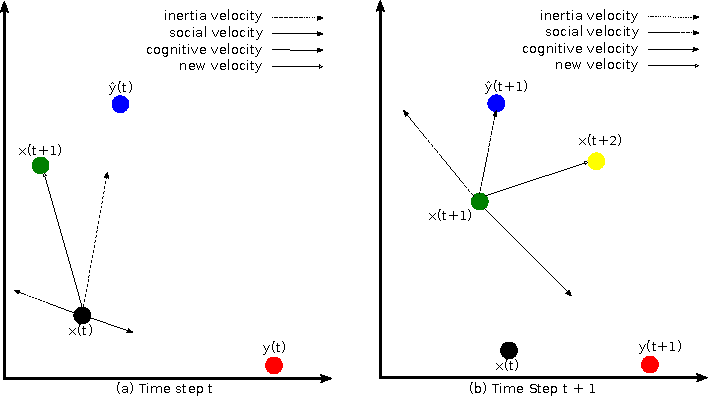
\includegraphics[width=4.5in,height=2.5in]{./pictures/geovelocity.pdf}}
	\caption{Visual particle velocity update \cite{SOSwarm,FundamentalSwarm,CompuIntelligenceIntro,PSOSelfHierarch}}
	\label{fig:particleVelocityUpdate}
	\end{center}
\end{figure}

As discussed earlier gbest is the best position the particle has occupied since the start of the algorithm. In the literature there are two defined methods of determining gbest. The most common method used is where gbest is the best position obtained by a particle in the swarm since the start of the algorithm; thus long-term knowledge dictates the best position found which favours exploitation \cite{CompuIntelligenceIntro,FundamentalSwarm}.

The second method of determining the gbest is the best particle position occupied by any particle in the swarm, in the \emph{current} iteration of the algorithm; thus short-term knowledge dictates the best position found which favours exploration \cite{CompuIntelligenceIntro,FundamentalSwarm}.

Most of the literature has concentrated on the velocity of the particle because it is the main function performing the optimisation. In research done by Ratnaweera et al.\cite{PSOSelfHierarch} particle positions in the solutions space are continually monitored. If the particle appears to be stagnant in the solution space, the velocity is first updated, and then the particle is reinitialised with a random position. The new position of the particle is then updated with the new velocity, thus knowledge of the discarded particle is retained by using the velocity it had\cite{PSOSelfHierarch}.

In research done by Kalivarapu et al. \cite{PSOPheromones} a PSO algorithm is developed that seeks to incorporate the pheromone notion of ACO algorithms into the velocity updating of particles. The premise of the method is to allow greater sharing of information about promising areas between particles. The algorithm developed by the authors achieved promising results, with it in certain cases finding solutions faster and also better solutions than other PSO algorithms \cite{PSOPheromones}. 

Other research done by Monson and Seppi \cite{adaptPSO} is more concerned with how the particle is presented. In the general PSO algorithm, particles have no physical form or volume and so particles in the swarm move through each other. The authors changed this in their algorithm by letting each particle have a radius around itself. This means that as particles move through the solution space and another particle at a certain time step occupies the same space, the particles are said to collide. As one would expect, when a collision occurs both particles are deflected into random directions \cite{adaptPSO}. At a greater expense of computational time due to constant collision detection, the PSO gains greater exploration in the solution space. 

Finally, in the research by Lenin and Monan a PSO algorithm is developed that is called the attract and repulse PSO (ARPSO). The algorithm continually monitors the solutions in the swarm. If it picks up that a certain percentage of the swarm is stagnating, it activates the repulse state. In the repulse state particles are repelled from other particles in the swarm, which facilitates greater exploration. After a certain number of iterations, the algorithm returns to its default state, where particles attract each other. The state of attraction facilitates exploitation \cite{PSOAttractRepulse}.
\subsubsection{Keeping velocity in check}
As can be observed in equation \ref{eq:velocityupdate} the new velocity is added to the old velocity. The velocity of particles can get very large, especially for those particles that are far from the pbest and gbest positions. Large velocities are necessary for early exploration. 

Velocities should be kept in check since if a particles velocity becomes too large, it can overstep the search spaces boundaries and produce infeasible solutions \cite{FundamentalSwarm}. Thus the velocity of a particle needs to be bounded to ensure that its movement with in the search space stays within acceptable bounds. One of the means to bound the velocity of a particle is by applying equation \ref{eq:velocityclamp}. The equation is applied on the velocity before its position is updated\cite{FundamentalSwarm}.
\begin{align}
	\vec{v_i}(t+1) &=
	\begin{cases}
	\vec{v'_i}(t+1), &\text{if $\vec{v'_i}(t+1) < \vec{V_{max}}$}\\
	\vec{V_{max}}, &\text{if $\vec{v'_i}(t+1) \geq \vec{V_{max}}$}
	\end{cases} \label{eq:velocityclamp}\\
	\vec{V_{max}} &= \delta(\vec{x_{max}} - \vec{x_{min}})
\end{align}
In equation~\ref{eq:velocityclamp} $\vec{v'_i}$ is calculated using equation~\ref{eq:velocityupdate} for the global PSO. Where $\vec{V_{max}}$ is the maximum allowed velocity and $\delta \in (0,1]$. The values $\vec{x_{max}}$ and $\vec{x_{min}}$ are the respective minimum and maximum position vectors in the domain the algorithm is being applied to \cite{FundamentalSwarm}. The value of $\delta$ is very problem dependent and must be carefully chosen to maximise the exploration-exploitation trade-off \cite{FundamentalSwarm}. The use of velocity clamping is not mandatory and should be considered only if the problem requires it\cite{FundamentalSwarm}. Finally there is no guarantee that velocity clamping will prohibit velocities becoming too large\cite{FundamentalSwarm}. There is still a chance, just to a smaller extent\cite{FundamentalSwarm}.

Velocity clamping is not the only developed means by which  the exploration-exploitation trade-off of the PSO can be control. Consider the case when an object moves with a certain velocity it carries momentum. If the object were to suddenly change direction, momentum would for a certain period still move the object in the previous direction. Inertia weight seeks to add type of behaviour to the particles of the PSO algorithm. The velocity update equation with added inertia is formulated in equation \ref{eq:inertia} \cite{FundamentalSwarm}.
\begin{equation}
\vec{v_i}(t+1) = w\vec{v_i}(t) + c_1\vec{\phi}_1(t)[\vec{pbest}_i - \vec{x}_i(t)] + c_2\vec{\phi}_2(t)[\vec{gbest}_i - \vec{x}_i(t)]\label{eq:inertia}
\end{equation}
Inertia ($w$ in equation \ref{eq:inertia}) was added to the general velocity update equation in an attempt to control the exploration and exploitation of the PSO as well as eliminate the need for velocity clamping\cite{FundamentalSwarm}. Although the inertia component did succeeded in enabling the control of the PSO's exploration-exploitation in the search space, the need for velocity clamping could not be eliminated\cite{FundamentalSwarm}.

For values of $w > 1$ , the inertia of the particle is increased. With increased the particle will explore more but it also more likely to leave the boundaries of the search space leading to infeasible solutions \cite{FundamentalSwarm}. 

When $w < 1$ and depending on the values of $c_1$ and $c_2$ each time a particles velocity is updated a certain amount of momentum is lost. The particle seems to slow down, allowing it to exploit the current solution space in finer detail \cite{FundamentalSwarm}. This is not always the case, as $w < 1$ can also lead to the particles in the swarm diverging never to converge on an optimal solution.

To allow for a greater trade-off between exploration and exploitation, the inertia value can be made dynamic. Exploration is favoured early on in an optimisation algorithm and  exploitation later on the algorithm when it is near an optimum; thus various methods that are either linear decreasing or non-linear decreasing have been developed that modify the inertia component as the algorithm moves around in the solution space \cite{CompuIntelligenceIntro,FundamentalSwarm}.

Finally, a similar inertia type component was developed from the analysis of particle dynamics \cite{FundamentalSwarm}. This new component is called the \emph{constriction coefficient} and, like the inertia above, also modifies the velocity update equation slightly\cite{adaptPSO,FundamentalSwarm,CompuIntelligenceIntro}. 

This modification can be observed in equation \ref{eq:velocityconstriction}, which is the standard velocity equation with the constriction coefficient. The constriction coefficient is formulated in equation \ref{eq:constriction}\cite{adaptPSO,FundamentalSwarm,CompuIntelligenceIntro}.
\begin{align}
v_i(t+1) &= \chi[v_i(t) + c_1\phi_{1}(t)[pbest - x_i(t)] + c_2\phi_{2}(t)[gbest - x_i(t)]]\label{eq:velocityconstriction}\\
\chi &= \frac{2\kappa}{\lvert 2 - \phi - \sqrt{\phi^2 - 4\phi}\rvert}\label{eq:constriction}
\end{align}

The constriction coefficient is represented by the value $phi$. The constriction coefficient evaluates to an ever-decreasing value between $[0,1]$. By using the constriction coefficient the PSO algorithm is also guaranteed to converge for values of $phi \geq 4$ and $\kappa \in [0,1]$. As with the inertia discussed above, high values of $\kappa$ allow for greater exploration and slow convergence, whereas low values of $\kappa$ force the algorithm to exploit the solution space and converge quickly \cite{adaptPSO,FundamentalSwarm,CompuIntelligenceIntro}.

\subsection{Flow of the Algorithm}
The general concepts that are evident in the PSO algorithm have been covered. Using these concepts a general overview will now be given of the PSO algorithm flow using algorithm~\ref{alg:PSO} as a reference point. Note that for the algorithm presented a start neighourhood topology is used and the algorithm is applied on a minimisation problem.
\begin{algorithm}[H]
\caption{Basic Global Particle Swarm Optimisation Algorithm\cite{CompuIntelligenceIntro}}
\label{alg:PSO}
	\begin{algorithmic}[1]
		\State Initialize $s_n$ swarm
		\While{Stopping condition not met}
			\For{each particle $p_i \leftarrow 0$ in $s_n$}
				\State Evaluate particle with fitness function $f(p_i)$
				\If{$f(p_i) \leq pbest(p_i)$}
					\State personal best of $p_i$ to $f(p_i)$
				\EndIf
				\If{$f(p_i) \leq f(gbest)$}
					\State $gbest \leftarrow f(p_i)$
				\EndIf
			\EndFor
			\For{each particle $p_i \leftarrow 0$ in $s_n$}
				\State update velocity of $p_i$ with equation~\ref{eq:velocityupdate}
				\State update position of $p_i$ with equation~\ref{eq:positionupdate}
			\EndFor
		\EndWhile
	\end{algorithmic}
\end{algorithm}

The PSO algorithm starts off by initialising the swarm of particles. Each particle is randomly assigned a certain position in the problem space. After the swarm has been initialised the algorithm enters the optimization or search phase, which starts in line 2.

Before the swarm can start moving around in the problem space, it first needs to determine the gbest particle as well as each particle's own pbest position. Therefore as can be observed in line 3, each particle's current fitness $f(p_i)$ is determined using a problem-specific fitness function. The fitness determines the lucrativeness of the current position a particle occupies in the problem space.

Once the fitness of a particle's position is calculated, the algorithm needs to determine whether the current position of the particle is its pbest since the algorithm started. This comparison can be seen occur in line 5. 

If the fitness of the currently held position is indeed better than the previous personal best of the particle, then the new position is remembered as the personal best for that particular particle, as can be observed in line 6.

Regardless of whether the personal best of a particle has been updated or not, the algorithm performs another comparison also utilising the calculated fitness of the current position of the particle. The algorithm uses this fitness to also determine whether the current position of the particle is the best in the \emph{entire} swarm, i.e. whether it is  the \emph{global} best (gbest). This comparison occurs in line  8.

If the position of the particle is indeed the best position in the entire swarm, the algorithm replaces the current gbest with the position of the current particle being evaluated, as seen in line 9.

After the swarm has been evaluated, each particle should have a personal best and the swarm should have a global best. The swarm is therefore ready to move around in the problem space, which occurs in algorithm~\ref{alg:PSO} from lines 12 -- 15.

For each particle in the swarm the algorithm determines the particle's new velocity, as can be observed in line 13. The velocity of a particle is calculated using equation~\ref{eq:velocityupdate}. 

Once the velocity of a specific particle has been calculated, the particle is ready to move to a new position. Moving a particle from its current position to a new position using the calculated velocity is done by applying equation~\ref{alg:PSO} and occurs in line 14 in algorithm~\ref{alg:PSO}.

After the whole swarm has been moved, the algorithm continues to the next iteration to evaluate the new positions. This process occurs until certain stopping criteria are met.


\subsection{PSO on the FAP}
\label{sec:psoonfap}
The PSO algorithm is also a relatively new algorithm and has been applied to only a handful of NP-Complete problems, including the FAP. In this dissertation the PSO algorithm will be utilized on the FS-FAP to try and produce optimal solutions. 

Only two groups have conducted research where the PSO has been applied to the FAP to produce a near optimal solution. The research concentrated on the MS-FAP variant of the FAP, and so the aim of their algorithm was to reduce the span of frequencies used. The problem this dissertation is concerned with is the FS-FAP where the amount of interference generated needs to be minimised. 

To date, no PSO algorithm has been designed to operate on the FS-FAP variant. Therefore, the interest in the research mentioned above is more to do with how the authors went about encoding a particular frequency plan as a position for a particle, than with the actual optimisation procedure.

In the research presented by Elkamchouchi et al.\cite{EgyptFAPPSO} a PSO algorithm is applied to produce optimal solutions for the MS-FAP. The way the authors went about assigning frequencies in their algorithm is known as frequency exhaustive assignment (FEA).
This method works by first generating a list of calls, called a \emph{call list}, denoting calls that occur in the system\cite{EgyptFAPPSO}. 

The FEA method then iterates over the calls in the list and assigns the lowest possible frequencies to the calls without violating interference constraints\cite{EgyptFAPPSO}. The authors note that the specific frequency that is assigned to a particular call depends heavily on the order the calls are in the list\cite{EgyptFAPPSO}.

Because of the success of the PSO on the MS-FAP, for this dissertation the PSO algorithm was selected as the primary means by which to address the FAP.

The algorithm also makes extensive use of knowledge gained by the various particles as they search the problem space. Depending on the values used for $w, c_1$ and $c_2$, a particle does not only keep personal history (with pbest), but the swarm as a whole keeps a history of the best particle (neighbourhood best). Thus with regard to FAP, it is possible that even though a particle might be in an overall bad position, it might have some small bit of good knowledge being overshadowed by bad knowledge. Through the extensive use of historical knowledge good information is more likely to be shared or kept slightly longer in the algorithms collective knowledge.

For this current research the PSO was applied to the FS-FAP on the COST259 benchmark problems. The approach by the authors in the above literature could not be used. FS-FAP is concerned with interference generated and there are some constraints which cannot be broken which are mentioned in section~\ref{sec:COST259} page~\pageref{sec:COST259}. In contrast with MS-FAP, the performance measure is explicitly the number of constraints violated not interference.

\section{Summary}
\label{sec:SISummary}
In this chapter three swarm intelligence algorithms were discussed. The general flow of the ant colony optimisation algorithm was described with the help of a pesudo code as well as how the algorithm came about. The defining characteristics of the algorithm were identified and a literature review was given of the ACO being applied to the FAP.

The second swarm intelligence algorithm was the artificial bee colony optimization algorithm. How the algorithm was developed and how it performs its search in a problem space were explained. A diagram also outlined the general flow of the ABC algorithm.

A series of defining characteristics was explained. Each characteristic is a defining attribute of the algorithm that makes it unique with regard to other algorithms. No literature is available on the algorithm being applied to the FAP since to date no research has been conducted on such an ABC algorithm.

This chapter concluded with the most important algorithm, which is used in this dissertation on the FAP, namely the particle swarm optimization algorithm. The flow of the PSO algorithm was described in \ref{alg:PSO}. Furthermore, characteristics that make the algorithm unique were explained, and a literature review was given of the PSO algorithm being applied to the FAP.
